\section{作业及答案：结构力学基础与技巧班第6次作业及答案（组合结构）}
\begin{analysisbox}
先拆分梁、桁架、刚架等子结构，连接点处作用力成对出现。对组合结构求解时应从约束较少或可独立平衡的部分开始。
\end{analysisbox}
\subsection*{第 1 页转写}
研究生入学考试辅导丛书结构力学（第二版）

根据结构与荷载特点，尽量利用简捷的方法求出结构的弯矩图。（武汉理工大学2010）

(a)

图2-162

三、练习题

2-33图2-163所示结构中杆AB的轴力为（

）。（哈尔滨工业大学2011）

A.0

B. 0.894 Fp

C. -0.5Fp

D. -Fp

2-34对图2-164所示结构，作受弯杆件的弯矩图，算出各链杆的轴力（标注在杆件

旁边）。（北京交通大学2010）

图2-163

图2-164

2-35

对图2-165所示结构作弯矩图，并求杆件1的轴力。（广州大学2011)

2-36

试作图2－166所示结构的弯矩图、剪力图、轴力图。（哈尔滨工业大学2010）

2-37

作图2-167所示结构的弯矩图。（重庆大学2010）

2-38

作图2-168所示结构的弯矩图。（重庆大学2012）

2-39

作图2－169所示结构的弯矩图，并求桁架杆件的轴力。（广州大学2007)

86
\begin{figure}[H]\centering
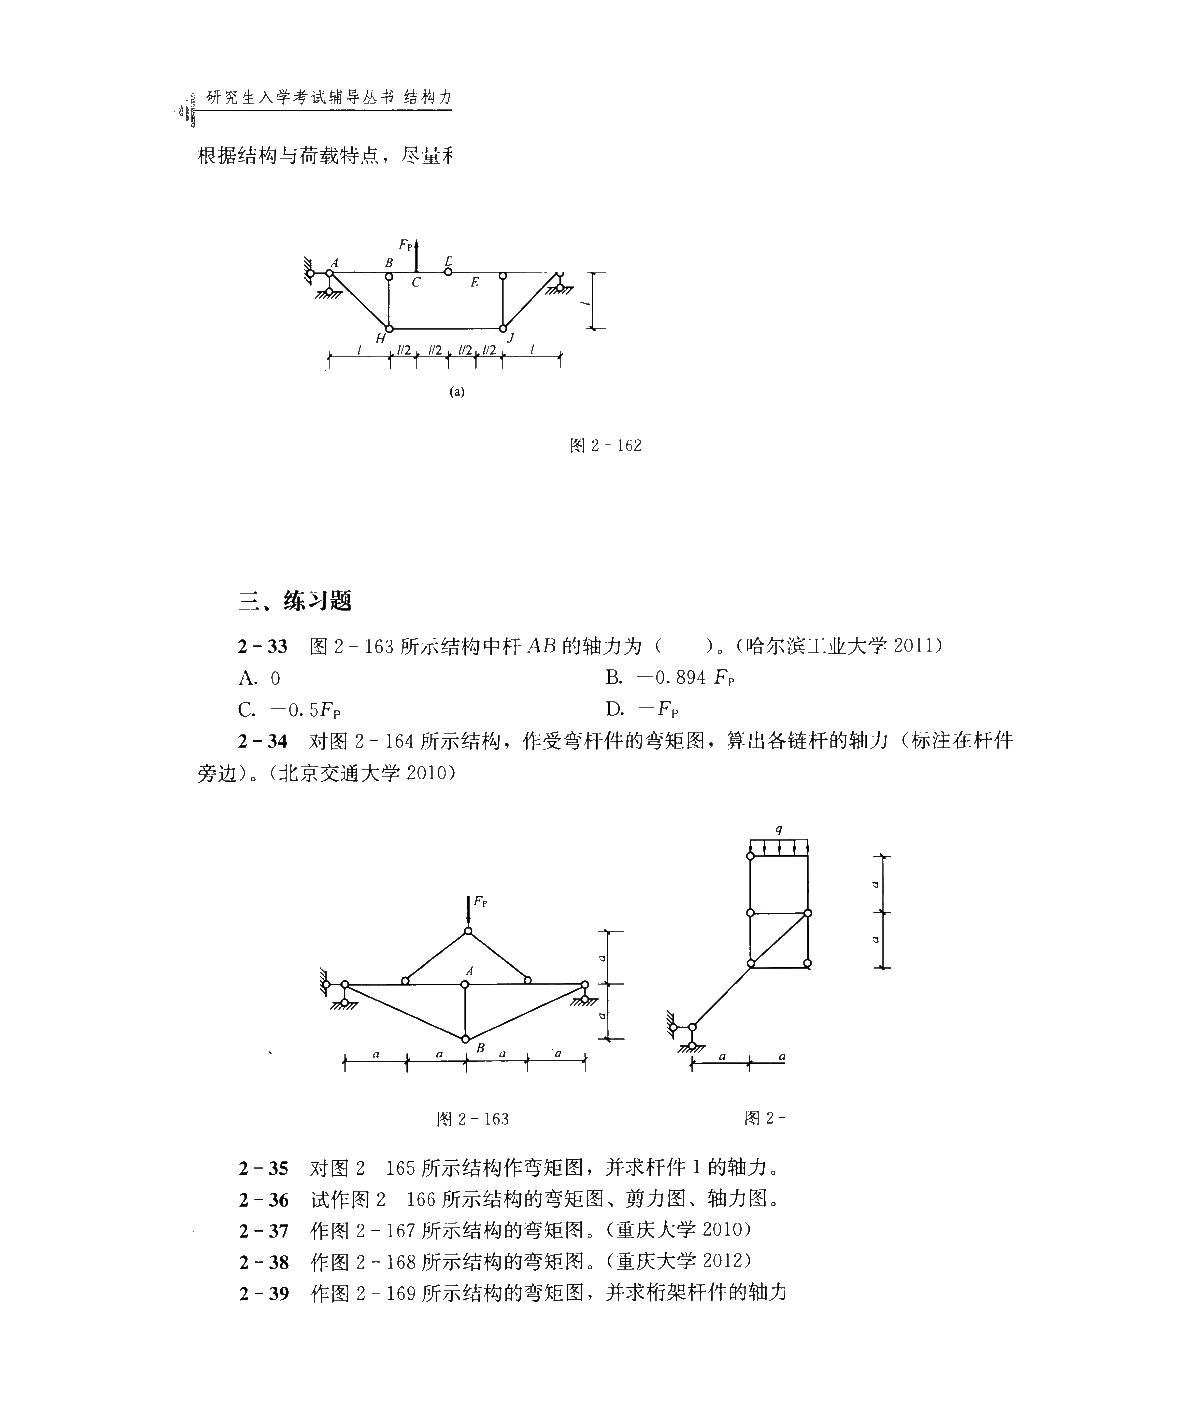
\includegraphics[width=0.92\textwidth]{figures/src09_p001.jpg}
\caption{结构力学基础与技巧班第6次作业及答案（组合结构） 第 1 页清理图形页}
\end{figure}
\subsection*{第 2 页转写}
Fp

20kN/m

20kN

4m

图2-165

图2-166

图2-167

2kN/m

Fp!

4m

图2-168

图2-169

四、练习题答案

2-33

C.

2 - 34

答案见图2-170。

2-35

FNl=一2ql；弯矩图见图2-171。

2-36

弯矩图、剪力图、轴力图如图2-172（a)、（b）、（c）所示。

M图、FN图

M图

图2-170

图2-171
\begin{figure}[H]\centering
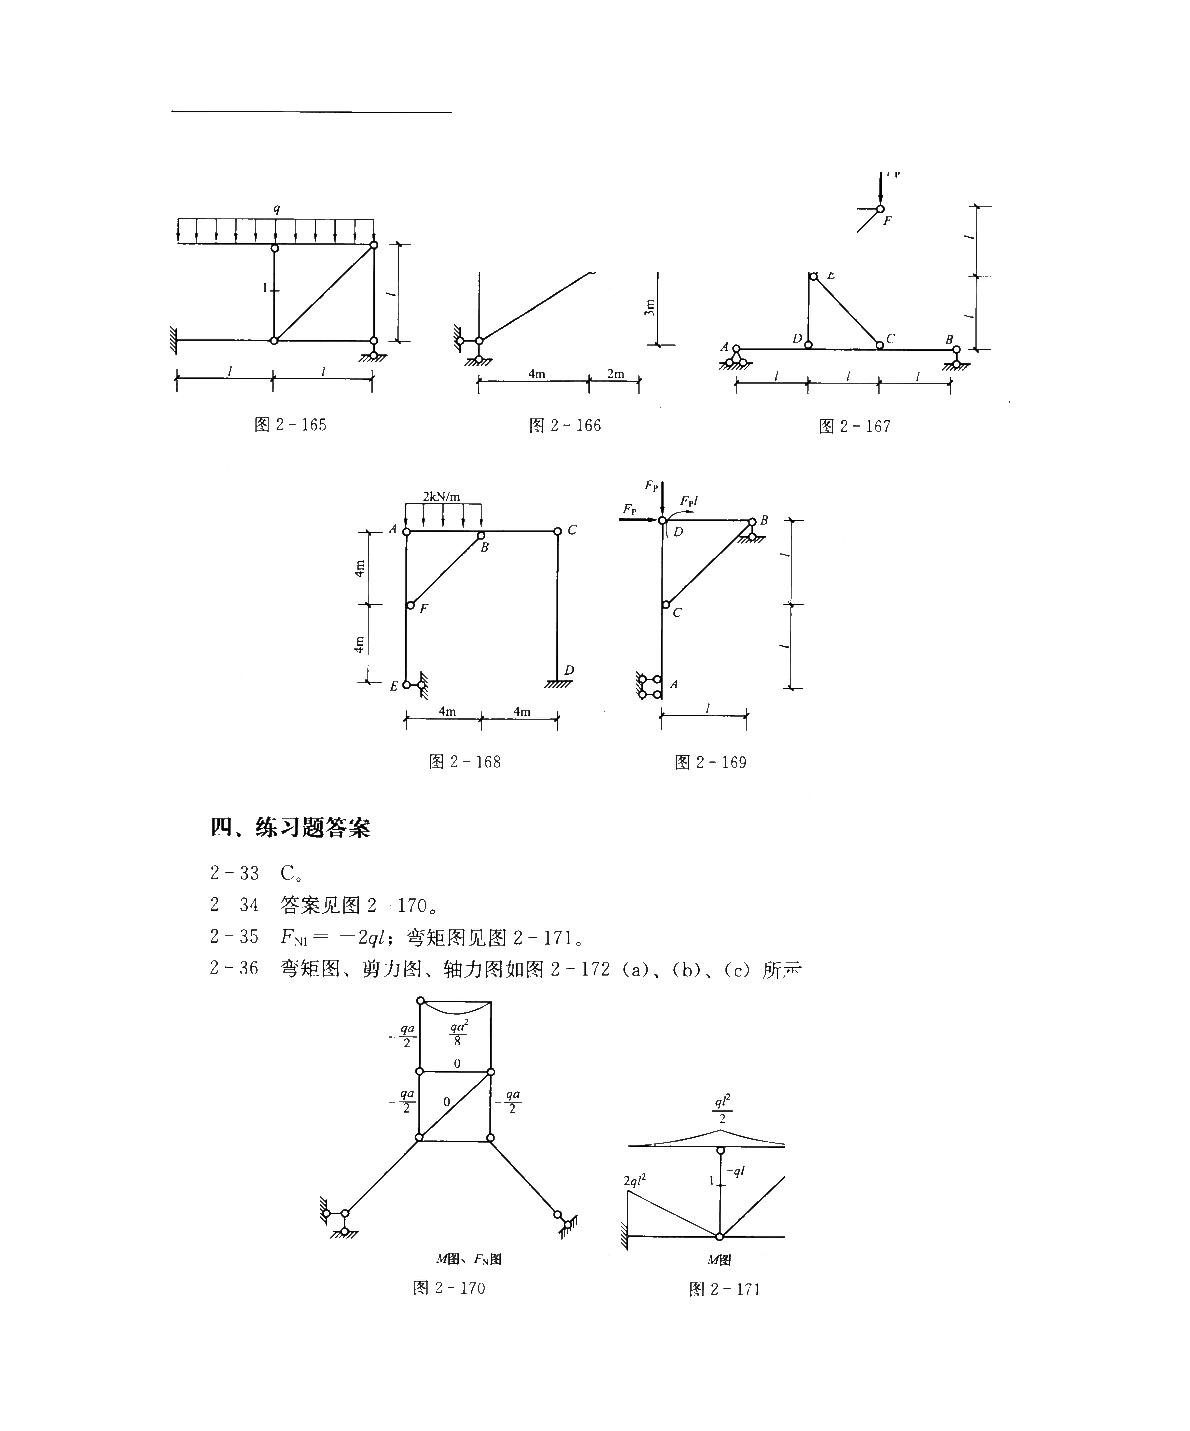
\includegraphics[width=0.92\textwidth]{figures/src09_p002.jpg}
\caption{结构力学基础与技巧班第6次作业及答案（组合结构） 第 2 页清理图形页}
\end{figure}
\subsection*{第 3 页转写}
研究生入学考试辅导丛书结构力学（第二版）

140

30

40

20

140

50

30

350

FQ图(kN)

FN图(kN)

(b)

(a)

(c)

图2-172

2-37

弯矩图如图2-173所示。

2-38

弯矩图如图2-174所示。

2-39

弯矩图如图2-175所示。

Fp!

Fp!

32

24

48

2Fpl

M图

图2-174

图2-173

图2-175

第四节

三铰拱

、拱的受力特点

（1）在竖向荷载作用下产生水平推力。

（2）因为水平推力的存在，使三铰拱的弯矩比相应简支梁的弯矩小。

（3）在竖向荷载作用下，梁的截面没有轴力，而拱的轴力较大，且一般为压力，因此，

拱比梁更便于利用抗压性能好而抗拉性能差的材料。

二、三铰拱在竖向荷载下的计算公式

1.支座反力公式

(1平拱［[见图2-176（a)］

88
\begin{figure}[H]\centering
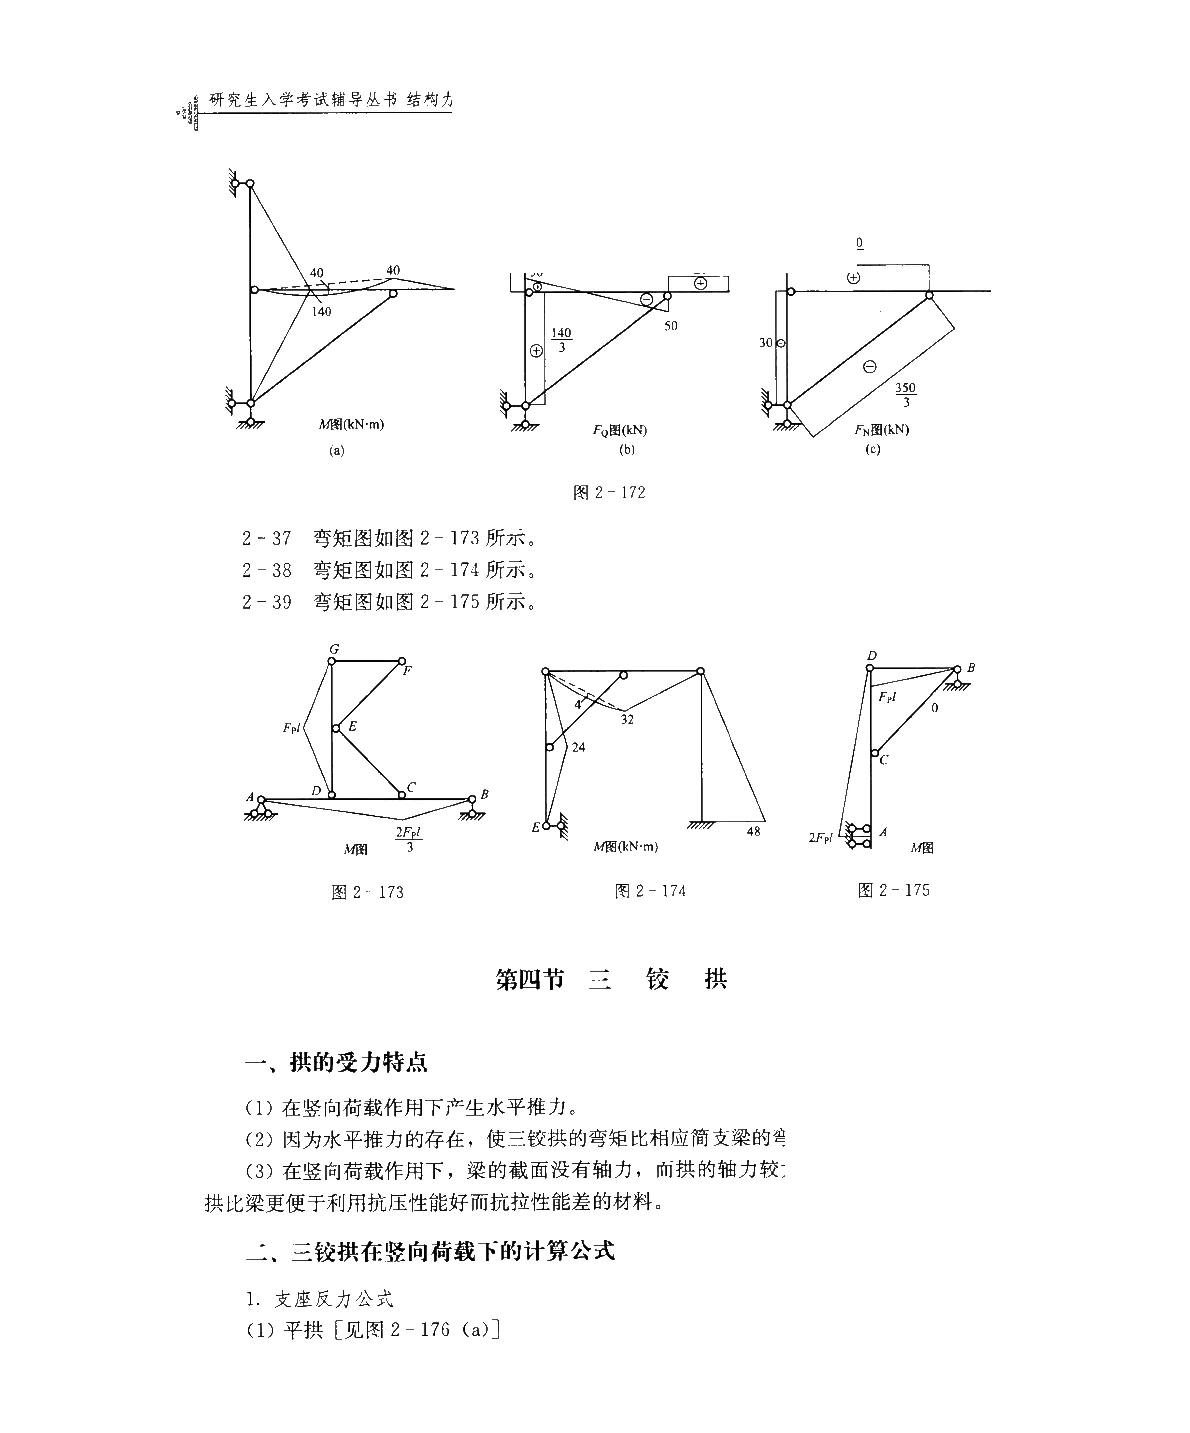
\includegraphics[width=0.92\textwidth]{figures/src09_p003.jpg}
\caption{结构力学基础与技巧班第6次作业及答案（组合结构） 第 3 页清理图形页}
\end{figure}
